%==================================================================================================
\FloatBarrier
\chapter{Implementation of the neuroevolution}
This chapter aims to describe the assumptions and implementation details of the neuroevolution 
algorithm developed in this project. 
While the description takes into account the target model functioning on the robot, 
in this chapter the attention is focused on a higher level of abstraction. 
The created algorithm should be able to operate largely in isolation from the specific target 
implementation.



%==================================================================================================
\FloatBarrier
\section{Observation-decision-reaction model}

In each evolutionary model, the concepts of an individual, environment, and fitness function 
should be clearly defined. 
In the case of a neural network, the concept of an individual must take into account the 
manner of interaction with the environment and the representation of the genotype.
\begin{figure}[htb] 
	\centering
	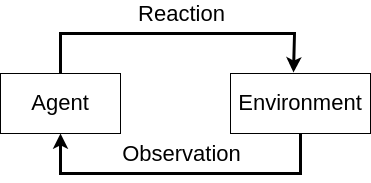
\includegraphics[width=0.6\textwidth]{figures/agent_environment}
	\caption{Interaction between agent and environment in used model.}
	\label{fig:agent_environment}
\end{figure}

Due to previous experience in robotics and multi-agent systems, it was decided to use a model 
based on the concept of an agent interacting with the environment through the 
observation-decision-reaction cycle. 
The relationship of the model elements is illustrated in Figure \ref{fig:agent_environment}.
The decision is sometimes referred to as the correlation, but this is more true of older works.
In this model, the agent acquires  information about the environment through observation and 
influences it through reaction. 
Since time is assumed to be a discrete variable, the observation at time $t_{i}$ corresponds to the 
state of the environment resulting from the reaction at time $t_{i-1}$. 
For a more effective description, another layer of abstraction is introduced, separating the 
decision system (correlator) from the specific features of the environment using receptor and effector 
objects. 
The internal structure of the agent described in this way is shown in Figure \ref{agent_internal}.
\begin{figure}[htb] 
	\centering
	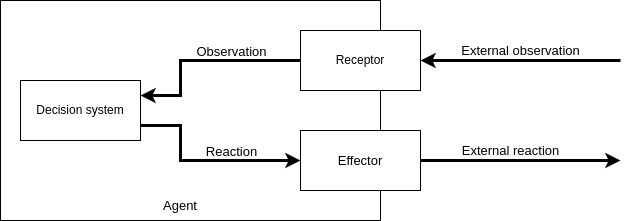
\includegraphics[width=0.9\textwidth]{figures/agent_receptor}
	\caption{Internal model of agent with enviroment interaction endpoints.}
	\label{fig:agent_internal}
\end{figure}

In such a model, we distinguish between internal and external observations, and the same applies 
to the reaction. Internal representations are independent of the physical implementation of the 
receptors and effectors. 
This is a significant advantage as it allows you to transfer decision systems from simulation to 
physical environments.

In the described project, the role of the receptor and the effector will be played by objects 
implementing the abstract EnvironmentEndpoint class shown in the listing

\begin{lstlisting}[language=C]
struct EnvironmentMetadata{

	enum ErrorCode{
		ENV_ERR_OK = 0, 
		ENV_ERR_UNKNOWN = 1 
	};

	int cycle;
	double reward;
	int running;
	ErrorCode error_code;
	std::string error_msg;
};

template<class Numeric> class Environment{

	virtual std::vector<Numeric> get_observation() const = 0;

	virtual void send_reaction(const std::vector<Numeric> &reaction) const = 0;

	virtual EnvironmentMetadata get_metadata() const = 0;

	virtual bool provides_learning_metadata() const = 0;

};
\end{lstlisting}

The classes inheriting from Environment must provide the implementation of the 
get\_observation and send\_reaction functions as both the receptor and the effector. 
In both cases, the internal representation of the observations and reactions is a vector of 
numerical values. A more precise definition of the numerical value in terms of this project is 
given in the section dedicated to this.
In addition to the basic interaction of the agent with the environment, objects belonging to 
this class also provide access to the metadata necessary for the operation of the genetic 
algorithm and the agent's supervisor.
In the case of a supervisor, this information is whether the point of interaction with the 
environment is working and whether there was an error in the last cycle. 
As for the information for the genetic algorithm, it is primarily a reward given for the agent's 
reaction in the last cycle. 
Not every point of interaction with the environment provides this information, it concerns only 
the simulation, therefore the objects of this class also provide the provides\_learning\_metadata 
function, which informs about whether the mentioned functionality is available.


%==================================================================================================
\FloatBarrier
\section{Representation of a network graph}

Before starting work on the implementation of the target model, a more conventional model, 
and thus easier to modify and analyze, should be created.
However, already at this stage, the limitations related to the target implementation must be 
taken into account, and they are as follows:
\begin{enumerate}
	\item Possibility to use any representation of numerical values in neural network operation.
    \item Limiting the available types of activation functions to a linear, rectifier, 
	unipolar and bipolar.
    \item Limiting the available types of aggregation functions to sum, product, minimum 
	and maximum
\end{enumerate}
To implement the first limitation, it was decided to use the template mechanism available in C++.
Thanks to this, it became possible to replace a specific implementation of a numerical value with
an abstract template called Numeric.

The compiler puts the selected implementation of a numeric type into the compilation process 
and generates the appropriate implementations of all classes and functions. 
Exactly what features an implementation of a numeric type must have been described in the 
\textbf{SUBSECTION REFERENCE} section.

The implementation of the second and third constraints is trivial and comes down to 
enumeration definitions containing only available functionalities and then selecting functions 
based on them. 
Note that the activation and aggregation functions must be defined for all implementations of 
the numeric type.
Another problem is the representation of individual neurons and their interactions. 
This problem has indeed been solved in many ways, but the selection of the correct representation 
largely depends on the application.
For example, for implementation using graphics card vector processors and neural networks with 
clear layer breakdowns, it makes the most sense to represent each layer as a link weight matrix 
plus a threshold value. 
Thanks to this approach, obtaining the response of a given layer is represented as a single matrix 
operation and then the application of the function to all elements of the result vector. 
Both of these operations are highly optimized in the hardware layer of vector processors and enable 
quick recalculation of even very complex networks.

In the case of the hardware environment used in the discussed project, however, such an 
implementation is not recommended. 
Not only the matrix representation does not introduce any performance improvement due to the 
lack of hardware support for vector calculations, but it also forces the creation of densely 
connected networks, which causes a significant increase in computational and memory complexity 
concerning networks with a sparse network of connections.
Finally, it was decided to use a graph model based on the concept of modeling the signal flow 
through a neural network where the nodes represent the cell body (soma) and the connections of 
dendrites and axons. 
The connections only store information about the target cell to which they send the signal and 
the weight by which this signal will be multiplied. 
The entire aggregation and activation mechanism has been placed in the cell body. 
A more detailed description of these elements can be found in the sections dedicated to them.
\begin{figure}[htb] 
	\centering
	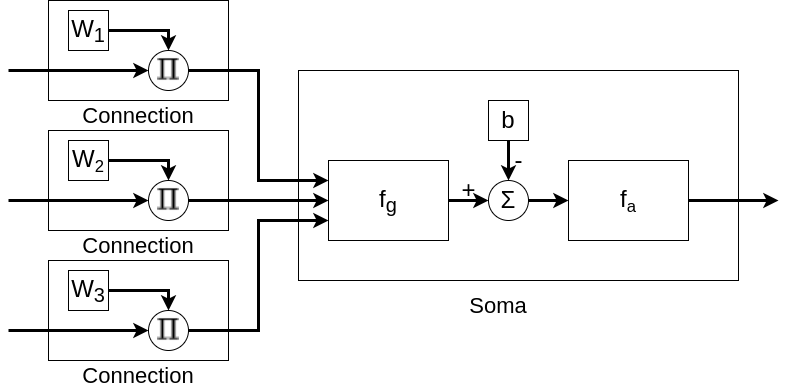
\includegraphics[width=\textwidth]{figures/signal_model}
	\caption{A signal flow trough neural cell.}
	\label{fig:signal_model}
\end{figure}

Figure \ref{fig:signal_model} shows the signal path for a neuron with three input connections. 
This type of visualization contains many repetitive elements that do not need to be shown 
when visualizing specific networks if the recipient is familiar with the assumptions 
of the model. 
Therefore, for the network visualization, the notation as in Figure 4 will be used, 
where the cell body is represented by a function block and the connection by an arrow. 
Both at the joints and the bodies, there are their identifiers with the notation 
resembling simple fractions. In the ``numerator'' there is a unique object 
identifier informing about its position in the topology, the pool of identifiers 
is separate for bodies and connections, therefore it is normal to have a connection 
with the same number as soma. In the case of a combination, only the weight is in the 
``denominator'', while in the cell body there are identifiers of the aggregation type 
(AGG), activation (ACT), and the threshold value (BIA).
\begin{figure}[htb] 
	\centering
	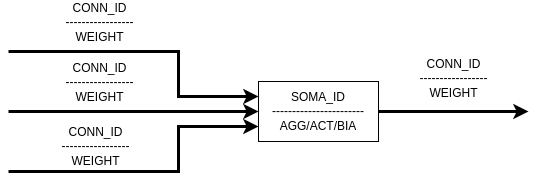
\includegraphics[width=0.8\textwidth]{figures/simple_mode}
	\caption{A simplified representation of neural cell.}
	\label{fig:simple_mode}
\end{figure}


The value of identifiers is displayed as an integer, weight, and threshold are treated 
as floating-point values regardless of the actual implementation of the numeric type. 
The aggregation field can take one of four values:  
\begin{itemize}
	\item SUM - sum 
	\item MUL - product 
	\item MIN - minimum 
	\item MAX - maximum 
\end{itemize}
The activation field can take one of four values:
\begin{itemize}
	\item LIN - linear
	\item REC - rectifier
	\item UNI - unipolar
	\item BIP - bipolar
\end{itemize}


%--------------------------------------------------------------------------------------------------
\FloatBarrier
\subsection{Numeric type - algebra definition}



%--------------------------------------------------------------------------------------------------
\FloatBarrier
\subsection{Soma}
The soma or cell body is the central part of the network. 
It is an object storing a state in the form of an activation potential and a cycle identifier. 
Each cell can have input and output connections, but two specific types of cells have an additional 
function
\begin{enumerate}
	\item sensory neurons - the value of observation is added to their activation potential and 
	it is from these neurons that the propagation of the signal in the network begins, 
	\item motor neurons - the activation values of these neurons are used to generate the 
	reaction vector.
\end{enumerate}
Neurons that have no additional function besides signal transmission are called interneurons, 
or internal neurons. 
It should be noted that due to the possibility of recursive connections, motor neurons are not 
necessarily the last elements of the signal sequence. 
The number of sensory and motor neurons depends on the task with which the network is measured, 
therefore they cannot be removed or added by topology-modifying mutations. 
In addition, these neurons must have information about which of the dimensions of observation or 
response they correspond to.


\begin{lstlisting}[language=C]
template<class Numeric> struct SomaTransfer{
	ActivationType activation; 
	AgregationType argregation;
	Numeric bias; 
};

template<class Numeric> struct SomaConnections{
public:
	std::vector< std::shared_ptr<Numeric> > outbound;
	std::vector< std::shared_ptr<Numeric> > inbound;
};

template<class Numeric> class SomaState{
	long cycle;
	Numeric activation_potential;

};

template<class Numeric> class Soma: public GenotypeDependant{
private:
	SomaRole role;
	SomaTransfer<Numeric> transfer;
	SomaConnections<Numeric> connections;
	SomaState<Numeric> state;

public:
	Soma(ActivationType activation, AgregationType agregation, SomaRole role, Numeric bias);
	Soma(const Soma<Numeric> &source);
	void add_signal(Numeric signal);
	void reset_activation_potential();
	Numeric activate() const;
	bool is_current_cycle(long current_cycel) const;
	void reset_state();
	void mutate_activation(std::vector<double> distribution);
	void mutate_agregation(std::vector<double> distribution);
	void mutate_bias(double factor);
	std::vector< std::shared_ptr< Connection<Numeric> > > get_outbound_connections() const;
	void connect_outgoing(std::shared_ptr< Connection<Numeric> > connection);
	void disconnect_outgoing(const Connection<Numeric> &connection);
	void connect_incoming(std::shared_ptr< Connection<Numeric> > connection);
	void disconnect_incoming(const Connection<Numeric> &connection);

};
\end{lstlisting}

As shown in listing , the cell body contains information about the current state of the cell and 
its configuration, as well as information about the topology based on the architecture of 
smart pointers.
Additionally, it contains an individual identifier referred to herein as a genetic marker that 
identifies the position of the cell in the topology. Cells with the same identifier can exist in 
two different networks as long as their positions in the relative topologies are the same. 
The type of aggregation, activation, and threshold value do not affect the marker.
The most important functions provided by Soma class objects are add\_signal and activate because 
they are used to model the signal flow through the cell. 
The function add\_signal attaches the incoming signal to the activation potential of the cell 
body according to the defined aggregation function. The activate function, on the other hand, 
returns the activation value for the current potential according to the determined activation 
function. 
Additionally, activation resets the activation potential and increments the cycle counter by one. 
This means that all signals reaching the neuron after activation will be counted to the potential 
in the next cycle.  This is important for modeling recursive connections.
Additionally, the cell provides functionalities related to genetic operators, such as crossing 
and mutation. 
A more detailed description of the functioning of these functions can be found in the section on 
the implementation of genetic operators.

%--------------------------------------------------------------------------------------------------
\FloatBarrier
\subsection{Connection}
The connection is a stateless element of the neural network topology. 
As its name implies, it connects the bodies of two cells and allows a signal to pass between them. 
The source of the signal is the activation value of the source cell which is then multiplied by 
the connection weight and sent to the target cell.
\begin{lstlisting}[language=C]
template<class Numeric> class Connection: public GenotypeDependant{

private:
	Numeric weight;
	std::shared_ptr< Soma<Numeric> > target;
	std::shared_ptr< Soma<Numeric> > source;

public:
	Connection();
	Connection(Numeric weight);
	Connection(const Connection& source);
	~Connection();
	void set_target(std::shared_ptr< Soma<Numeric>> target);
	void set_source(std::shared_ptr< Soma<Numeric>> source);
	Numeric pass_signal(Numeric signal) const;
	void mutate(double factor);
	Numeric get_weight() const;
	bool is_inhibitory() const;
	std::shared_ptr< Soma<Numeric> > get_target() const;
	std::shared_ptr< Soma<Numeric> > get_source() const;

};
\end{lstlisting}


As shown in the listing, the connection contains both weight and topology position information.
As with the cell body, topology information is realized using smart pointers. 
Another similarity is the presence of a unique genetic marker. These markers are separated from 
a separate pool than for cell bodies, therefore the connection and the body with the same 
identifier do not have to be related to each other in any way.


%==================================================================================================
\FloatBarrier
\section{Genetic operators}


%--------------------------------------------------------------------------------------------------
\FloatBarrier
\subsection{Initial population generation}
To create a new population with a sufficiently high degree of diversity, a pool of seed agents 
for the species is generated. 
The creation of such an agent is carried out by repeatedly triggering mutations that add cell 
bodies and connections to the base agent network model.
The base model contains only sensory and motor cells, the number of which is dictated by the 
type of receptors and effectors of the agent. 
These kinds of cells cannot be removed or added through the mutation process. 
The base model does not contain any connections and cannot by itself be used as an agent 
control network.
From the pool of seed agents, target agents are generated by using mutations that do not 
modify the topology, that is:
\begin{itemize}
	\item change of connection weight
	\item change of cell threshold
	\item changing the aggregation function of a cell
	\item changing the cell activation function
\end{itemize}
Mutations at this stage occur to a much greater extent than during the mutation stage in the 
main loop of the algorithm. 
Not only does a fixed number of mutations take place, but instead of randomizing the probability 
of their occurrence, all parameters have much higher values.
The result of this process is an agent population divided into species, each of which 
represents a specific topology.

%--------------------------------------------------------------------------------------------------
\FloatBarrier
\subsection{Calculating fitness values}
To perform the selection, it is necessary to establish the value of the agents' adaptation to 
the environment. 
For this purpose, a special environment is used that can evaluate the actions of the agent 
and award rewards for each of his reactions. 
The prizes may have a negative value, in which case they are referred to as penalties.
Each interaction of the agent with the environment is defined as an episode that has initial 
conditions, lasts a certain number of cycles, and ends when the stop condition occurs.
The universal condition of the stop is reaching the cycle limit, while for each environment, 
additional conditions are defined related to damage to the agent or the loss of the possibility 
of achieving the goal set for it.
The value of the agent's adjustment is the sum of the rewards over the entire period, 
therefore evolution, like its natural counterpart, will reward behavior that ensures survival, 
regardless of the specific goal of the agent.
This should be taken into account when determining the reward for achieving the goal, which must 
be higher than the possible combination of the remaining rewards obtained in the total number of 
cycles.
Even in that case, evolution may favor agents striving to achieve their goal as late as possible. 
One way around this problem is to add a penalty called "the pain of existence", which means that 
in each cycle the default reward is negative, and only taking some action to bring the agent 
closer to the goal can avoid the penalty.
Since the initial conditions and the transition between cycles contain elements of randomness, 
it is necessary to guide the agent through several episodes and then calculate the average adaptation. 
The elements of randomness are necessary because otherwise the neural network could only change 
and adapt to the specific training environment.
This would be extremely harmful as robotic agents are designed to operate in environments with 
low predictability and high levels of noise.

%--------------------------------------------------------------------------------------------------
\FloatBarrier
\subsection{Selection}
After the fitness of all agents in the population has been established, the selection of 
individuals that will enter the reproductive pool begins. As part of this project, the concept 
of the elite was applied, which means that the group of the best individuals will end up in the 
reproductive pool and will be transferred unchanged to the next generation. 
Due to the division into species in the implemented model, the presence of an individual of 
a given species also guarantees a place in the reproductive pool for a group of other individuals 
of a given species.
In the case of agents who are added to the pool due to the representation of the species in 
the elite, a roulette algorithm is used, while in the case of other agents, a combination of 
roulette and tournament algorithms is used.
In the first step of the algorithm, two species are selected, and a roulette algorithm functions 
here, the weights of which are the total adjustment of individuals of a given species. 
Then the roulette algorithm is called again for each of the species and a representative is 
selected on its basis. 
Representatives of both species are then subject to the tournament algorithm, and the one whose 
match has the higher value is added along with another individual of his species selected 
completely randomly to the reproductive pool.

%--------------------------------------------------------------------------------------------------
\FloatBarrier
\subsection{Crossover}
After the generation of a reproductive pool as part of the selection, crossbreeding occurs. 
Due to the use of the species disaggregated population model, there are several possible approaches 
to allowed parent combinations. 
\begin{enumerate}
	\item Free interspecies mating
	\item Can only be reproduced between related species
	\item No possibility of interspecies evaporation.
\end{enumerate}
Free association allows the greatest variety of topologies to be created, and at the same time, 
it is the least stable solution. 
This is the only variant that allows for the emergence of a new species in the process of 
crossing. 
As in the case of the NEAT implementation on which it was modeled, this variant will be used 
in this project.

%--------------------------------------------------------------------------------------------------
\FloatBarrier
\subsection{Mutation}
The new generation generated by crossbreeding is then mutated. Without this operator, 
it would be impossible for new information to appear in the model, 
but only to recombine existing settings.
In this work, we distinguish two types of mutations. The first is the transmittance mutation 
and the second is the topology mutation. 
As part of the transmittance mutation, the aggregation function, activation function, 
connection weight, or activation threshold can change.
If the aggregation and activation operators are modified, the new value is selected from a 
predefined pool according to the probability distribution specified in the configuration.
In case of mutation of numerical values
